\frame{\titlepage}
%INTRO:                                                                                  
%    - what is the project?                                                          DAN
%    - what is pcr and why is it important?
%    - what are primers?
%    - explain "simulation" (DO NOT SAY) to save time and money
%    - explain rules themselves    
\begin{frame}
	\frametitle{Project Outline}
	\begin{itemize}
		\item To develop a PCR primer design exercise to complement Molecular Methods lab course
		\item Will be used by Level 3 Life Sciences undergraduates in the lab and at home
		\item System must function as a portable, robust and interactive teaching tool
		\item Basic understanding of theory behind PCR and primer design required
	\end{itemize} 
\end{frame}    

\begin{frame}[fragile]
	\frametitle{What Is PCR?}
	\begin{itemize}
		\item Polymerase Chain Reaction
		\item Developed in 1983, by Kary Mullis
		\item Variety of real-world applications
		\item Process of amplifying a sequence of DNA several thousand times
		\item DNA double-stranded, made up of sequences of nucleotides, or bases, represented by \verb£a£, \verb£t£, \verb£g£ and \verb£c£
		\item Uses two smaller sequences at start and end of target sequence, heated to ``anneal'' to strand
		\item Enzyme called Taq polymerase synthesises complementary strand to target sequence
	\end{itemize}  
\end{frame}

\begin{frame}
	\frametitle{Primers}
	\begin{itemize}
		\item Shorter sequences of DNA, around 20 - 30 in length
		\item Forward and reverse primers, one at each end of the target sequence on opposite strand
		\item Must adhere to a number of design rules to ensure effectiveness
		\item Selecting such a sequence is the focus of the exercise
	\end{itemize}
\end{frame}

\begin{frame}
	\frametitle{Primer Rules}
	\begin{itemize}
		\item Melting temperature within 50 - 65\degree C
		\item Unique to the strand
		\item Ends in base \texttt{g} or \texttt{c}
		\item Bases do not repeat more than 3 times in a row
		\item Length between 20 and 30
		\item \texttt{gc} content between 40-60\%
		\item Must not self-anneal
		\item Must not anneal to other primers
	\end{itemize}
\end{frame}

\begin{frame}
\frametitle{Annealing}
\begin{figure}[!t]
  \begin{center}
    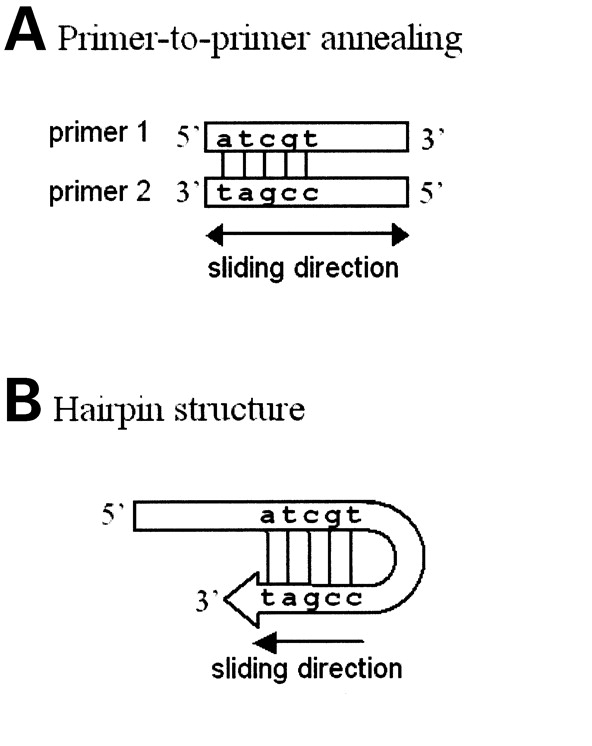
\includegraphics[width=0.6\textwidth]{./img/annealing.jpg}
  \end{center}
\end{figure}


\end{frame}     
